\section{Sorting Algorithms: histograms of single phases}
\label{appendix}

\subsection*{Pianosa}

\begin{figure}[h]
	\centering
	\subfloat[2 processors.]{\label{RxTxP-n2_quicksort}\includegraphics[width=0.42\textwidth]{plots/test_01_pianosa/RxTxP/n2_M1073741824_quicksort_pianosa_RxTxP}} 
	\hspace*{20pt}	
  	\subfloat[4 processors.]{\label{RxTxP-n4_quicksort}\includegraphics[width=0.42\textwidth]{plots/test_01_pianosa/RxTxP/n4_M1073741824_quicksort_pianosa_RxTxP}} 
	
	\centering
	\subfloat[8 processors.]{\label{RxTxP-n8_quicksort}\includegraphics[width=0.42\textwidth]{plots/test_01_pianosa/RxTxP/n8_M1073741824_quicksort_pianosa_RxTxP}} 
  	\hspace*{20pt}
  	\subfloat[16 processors.]{\label{RxTxP-n16_quicksort}\includegraphics[width=0.42\textwidth]{plots/test_01_pianosa/RxTxP/n16_M1073741824_quicksort_pianosa_RxTxP}} 
  	
	\caption{\textbf{Quicksort}. Histograms showing load balancing among processors in the different phases of Quicksort.}
	\label{RxTxP}
\end{figure}

\begin{figure}[h]
    \centering
    \subfloat[2 processors.]{\label{RxTxP-n2_bitonicsort}\includegraphics[width=0.38\textwidth]{plots/test_01_pianosa/RxTxP/n2_M1073741824_bitonicsort_pianosa_RxTxP}} 
    \hspace*{20pt}  
    \subfloat[4 processors.]{\label{RxTxP-n4_bitonicsort}\includegraphics[width=0.38\textwidth]{plots/test_01_pianosa/RxTxP/n4_M1073741824_bitonicsort_pianosa_RxTxP}} 
    
    \centering
    \subfloat[8 processors.]{\label{RxTxP-n8_bitonicsort}\includegraphics[width=0.38\textwidth]{plots/test_01_pianosa/RxTxP/n8_M1073741824_bitonicsort_pianosa_RxTxP}} 
    \hspace*{20pt}
    \subfloat[16 processors.]{\label{RxTxP-n16_bitonicsort}\includegraphics[width=0.38\textwidth]{plots/test_01_pianosa/RxTxP/n16_M1073741824_bitonicsort_pianosa_RxTxP}} 
    
    \caption{\textbf{Bitonicsort}. Histograms showing load balancing among processors in the different phases of Bitonicsort.}
    \label{RxTxP}

    \centering
    \subfloat[2 processors.]{\label{RxTxP-n2_bucketsort}\includegraphics[width=0.38\textwidth]{plots/test_01_pianosa/RxTxP/n2_M1073741824_bucketsort_pianosa_RxTxP}} 
    \hspace*{20pt}  
    \subfloat[4 processors.]{\label{RxTxP-n4_bucketsort}\includegraphics[width=0.38\textwidth]{plots/test_01_pianosa/RxTxP/n4_M1073741824_bucketsort_pianosa_RxTxP}} 
    
    \centering
    \subfloat[8 processors.]{\label{RxTxP-n8_bucketsort}\includegraphics[width=0.38\textwidth]{plots/test_01_pianosa/RxTxP/n8_M1073741824_bucketsort_pianosa_RxTxP}} 
    \hspace*{20pt}
    \subfloat[16 processors.]{\label{RxTxP-n16_bucketsort}\includegraphics[width=0.38\textwidth]{plots/test_01_pianosa/RxTxP/n16_M1073741824_bucketsort_pianosa_RxTxP}} 
    
    \caption{\textbf{Bucketsort}. Histograms showing load balancing among processors in the different phases of Bucketsort.}
    \label{RxTxP}
\end{figure}

\begin{figure}[h]
    \centering
    \subfloat[2 processors.]{\label{RxTxP-n2_samplesort}\includegraphics[width=0.38\textwidth]{plots/test_01_pianosa/RxTxP/n2_M1073741824_samplesort_pianosa_RxTxP}} 
    \hspace*{20pt}  
    \subfloat[4 processors.]{\label{RxTxP-n4_samplesort}\includegraphics[width=0.38\textwidth]{plots/test_01_pianosa/RxTxP/n4_M1073741824_samplesort_pianosa_RxTxP}} 
    
    \centering
    \subfloat[8 processors.]{\label{RxTxP-n8_samplesort}\includegraphics[width=0.38\textwidth]{plots/test_01_pianosa/RxTxP/n8_M1073741824_samplesort_pianosa_RxTxP}} 
    \hspace*{20pt}
    \subfloat[16 processors.]{\label{RxTxP-n16_samplesort}\includegraphics[width=0.38\textwidth]{plots/test_01_pianosa/RxTxP/n16_M1073741824_samplesort_pianosa_RxTxP}} 
    
    \caption{\textbf{Samplesort}. Histograms showing load balancing among processors in the different phases of Samplesort.}
    \label{RxTxP}

    \centering
    \subfloat[2 processors.]{\label{RxTxP-n2_mergesort}\includegraphics[width=0.38\textwidth]{plots/test_01_pianosa/RxTxP/n2_M1073741824_mergesort_pianosa_RxTxP}} 
    \hspace*{20pt}  
    \subfloat[4 processors.]{\label{RxTxP-n4_mergesort}\includegraphics[width=0.38\textwidth]{plots/test_01_pianosa/RxTxP/n4_M1073741824_mergesort_pianosa_RxTxP}} 
    
    \centering
    \subfloat[8 processors.]{\label{RxTxP-n8_mergesort}\includegraphics[width=0.38\textwidth]{plots/test_01_pianosa/RxTxP/n8_M1073741824_mergesort_pianosa_RxTxP}} 
    \hspace*{20pt}
    \subfloat[16 processors.]{\label{RxTxP-n16_mergesort}\includegraphics[width=0.38\textwidth]{plots/test_01_pianosa/RxTxP/n16_M1073741824_mergesort_pianosa_RxTxP}} 
    
    \caption{\textbf{Mergesort}. Histograms showing load balancing among processors in the different phases of Mergesort.}
    \label{RxTxP}
\end{figure}

\begin{figure}[h]
    \centering
    \subfloat[2 processors.]{\label{RxTxP-n2_kmerge}\includegraphics[width=0.38\textwidth]{plots/test_01_pianosa/RxTxP/n2_M1073741824_kmerge_pianosa_RxTxP}} 
    \hspace*{20pt}  
    \subfloat[4 processors.]{\label{RxTxP-n4_kmerge}\includegraphics[width=0.38\textwidth]{plots/test_01_pianosa/RxTxP/n4_M1073741824_kmerge_pianosa_RxTxP}} 
    
    \centering
    \subfloat[8 processors.]{\label{RxTxP-n8_kmerge}\includegraphics[width=0.38\textwidth]{plots/test_01_pianosa/RxTxP/n8_M1073741824_kmerge_pianosa_RxTxP}} 
    \hspace*{20pt}
    \subfloat[16 processors.]{\label{RxTxP-n16_kmerge}\includegraphics[width=0.38\textwidth]{plots/test_01_pianosa/RxTxP/n16_M1073741824_kmerge_pianosa_RxTxP}} 
    
    \caption{\textbf{4-way mergesort}. Histograms showing load balancing among processors in the different phases of 4-way mergesort.}
    \label{RxTxP}

    \centering
    \subfloat[2 processors.]{\label{RxTxP-n2_lbmergesort}\includegraphics[width=0.38\textwidth]{plots/test_01_pianosa/RxTxP/n2_M1073741824_lbmergesort_pianosa_RxTxP}} 
    \hspace*{20pt}  
    \subfloat[4 processors.]{\label{RxTxP-n4_lbmergesort}\includegraphics[width=0.38\textwidth]{plots/test_01_pianosa/RxTxP/n4_M1073741824_lbmergesort_pianosa_RxTxP}} 
    
    \centering
    \subfloat[8 processors.]{\label{RxTxP-n8_lbmergesort}\includegraphics[width=0.38\textwidth]{plots/test_01_pianosa/RxTxP/n8_M1073741824_lbmergesort_pianosa_RxTxP}} 
    \hspace*{20pt}
    \subfloat[16 processors.]{\label{RxTxP-n16_lbmergesort}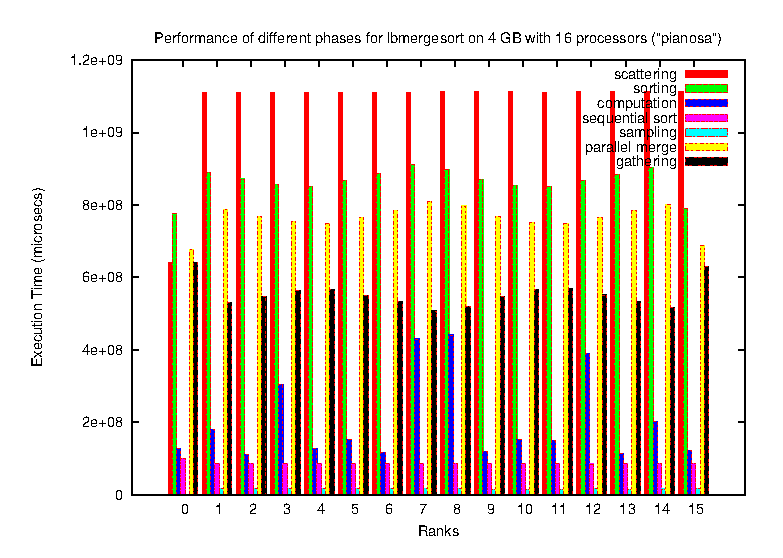
\includegraphics[width=0.38\textwidth]{plots/test_01_pianosa/RxTxP/n16_M1073741824_lbmergesort_pianosa_RxTxP}} 
    
    \caption{\textbf{Load-balanced mergesort}. Histograms showing load balancing among processors in the different phases of Load-balanced mergesort.}
    \label{RxTxP}
\end{figure}

\begin{figure}[h]
    \centering
    \subfloat[2 processors.]{\label{RxTxP-n2_lbkmergesort}\includegraphics[width=0.42\textwidth]{plots/test_01_pianosa/RxTxP/n2_M1073741824_lbkmergesort_pianosa_RxTxP}} 
    \hspace*{20pt}  
    \subfloat[4 processors.]{\label{RxTxP-n4_lbkmergesort}\includegraphics[width=0.42\textwidth]{plots/test_01_pianosa/RxTxP/n4_M1073741824_lbkmergesort_pianosa_RxTxP}} 
    
    \centering
    \subfloat[8 processors.]{\label{RxTxP-n8_lbkmergesort}\includegraphics[width=0.42\textwidth]{plots/test_01_pianosa/RxTxP/n8_M1073741824_lbkmergesort_pianosa_RxTxP}} 
    \hspace*{20pt}
    \subfloat[16 processors.]{\label{RxTxP-n16_lbkmergesort}\includegraphics[width=0.42\textwidth]{plots/test_01_pianosa/RxTxP/n16_M1073741824_lbkmergesort_pianosa_RxTxP}} 
    
    \caption{\textbf{Load-balanced Multi-way mergesort}. Histograms showing load balancing among processors in the different phases of Load-balanced Multi-way mergesort.}
    \label{RxTxP}
\end{figure}

\clearpage
 
 \subsection*{PCM}